\section{UML export}

In this section we will show you how you can create and view \emph{UML} diagrams from a \emph{Reprotool} project. You should already
have in your workspace a project named \emph{UML Export}. We will use this project in the current chapter. If you do not
have this project in your workspace, install the \emph{Reprotool example projects}. We use the
\emph{UML2 Tools} eclipse plugin for displaying the \emph{UML} diagrams.

\subsection{UML Use-Case diagram}
The use-case diagram contains information about the actors and use-cases in the project. The diagram shows the relationship between
actors and use-cases and the relationship between use-cases themselves.

Right-click on the \emph{umlExport.swproj} project file in the \emph{Project explorer} and select the \emph{Conwert SW project to UML use case
diagram} command. After that you should note a new file in the \emph{Project explorer} with the \emph{.swproj.uc.uml} file extension.
Right-click this file and select the \emph{Initialize Use Case Diagram} command. Now just click \emph{Finish}. An UML diagram should
fire up in a new editor instance. You should see the UML diagram similar to the one in this figure:

\begin{figure}[ht]
  \centering
  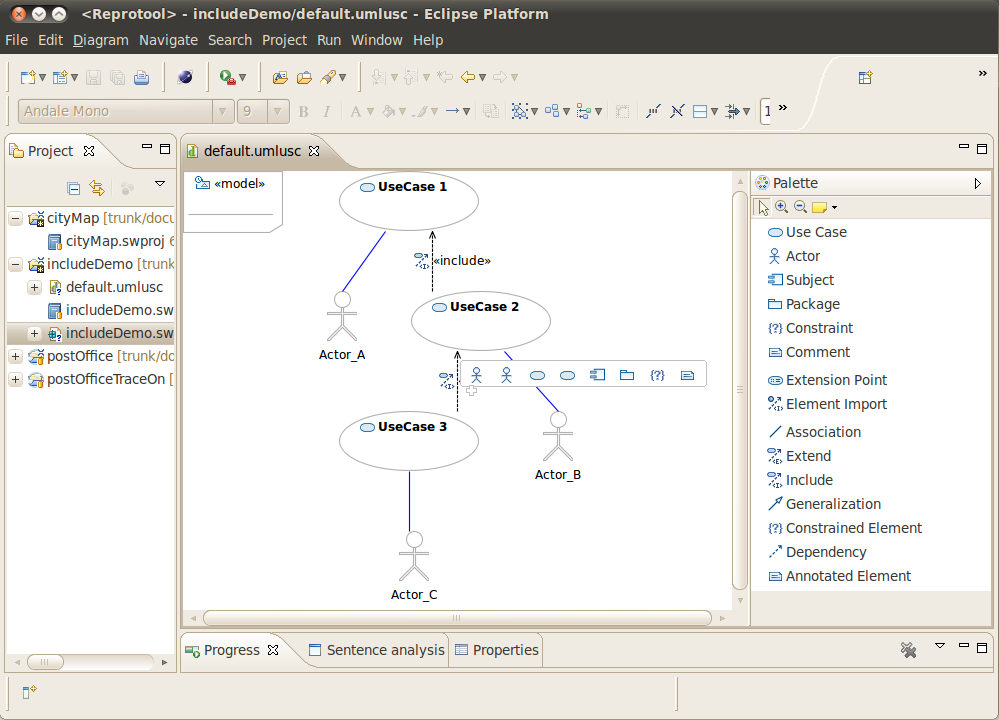
\includegraphics[height=250pt]{images/reprotoolUCDiagram}
  \caption{UML Use-case diagram of the \emph{UML Export} example project}
  \label{fig:reprotoolUCDiagram}
\end{figure}

\newpage

\subsection{UML Class diagram}
The \emph{UML Class diagram} contains the information about the actors in the software project and their actions. These actions can
be determined by running the linguistic analysis and if neccesary refined by manual analysis.

Right-click on the \emph{umlExport.swproj} project file in the \emph{Project explorer} and select the \emph{Conwert SW project to UML class
diagram} command. After that you should note a new file in the \emph{Project explorer} with the \emph{.swproj.class.uml} file extension.
Right-click this file and select the \emph{Initialize Class Diagram} command. Now just click \emph{Finish}. An UML class diagram should
fire up in a new editor instance. You should now face the UML class diagram similar to this one:

\begin{figure}[ht]
  \centering
  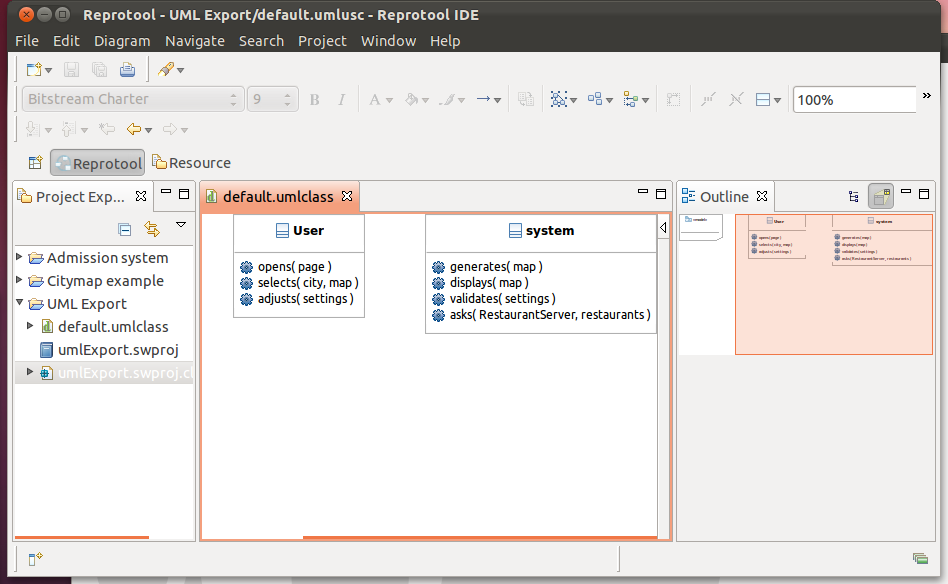
\includegraphics[height=250pt]{images/reprotoolClassDiagram}
  \caption{UML Class diagram of the \emph{UML Export} example project}
  \label{fig:reprotoolClassDiagram}
\end{figure}